\documentclass{softwaremanual}

\usepackage{titling}

% Figures and controlling packages
\usepackage{float}
\usepackage{wrapfig}

% logo for the title page
\newcommand{\swlogo}{{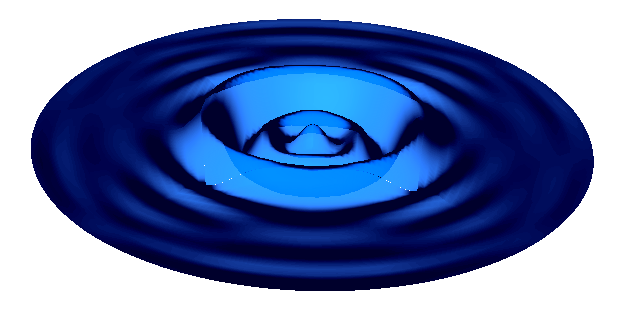
\includegraphics[width=0.25\textwidth]{images/shallowWater.png}}
}


\author{Joseph Schoonover}
\date{}

\begin{document}
\frontmatter
% Doing a custom title-page
\begin{titlingpage}
    
        \vspace*{2cm}

   % Setup up the main and sub-titles with the logo
   {\fontfamily{cmss}\selectfont
   \begin{center}
     \HUGE{\textbf{ Spectral Element Libraries in Fortran (SELF) }}\\

     \huge{\textbf{\textcolor{blue}{Shallow Water Equations}}}
   \end{center}
    }    
 
        \vspace{1cm}
        
        \begin{center}
         \swlogo
        \end{center}
        
        \vspace{2cm}
        
     \begin{center}
     
        %Do a subtitle here if you like
        {\fontfamily{cmss}\selectfont
        \huge{
           Reference Manual
        }
        
        \vspace{1.5cm}
        
        % Enter the author's name
        \textbf{
        \large{
           \theauthor 
         }}}
        
        \vfill
        
        
     \end{center}
        
    
\end{titlingpage}


{\fontfamily{cmss}\selectfont
\tableofcontents
}
\mainmatter

% Special Style
\pagestyle{myheadings}

\chapter{Equations and Discretization}
The inviscid shallow water equations are a system of coupled partial differential equations that is hyperbolic. The Nodal Discontinuous Galerkin Spectral Element Method (NDGSEM) is well suited for hyperbolic systems. It is highly accurate through its use of arbitrarily high order piecewise polynomial representation and exhibits minimal numerical dispersion and dissipation errors. It additionally allows for a flexible treatment of the geometry through the use of a structured or unstructured arrangement of \textit{spectral elements} that can represent boundaries through high order polynomial interpolants. The discretization yields dense and local matrix-vector multiplies for computing derivatives and only requires nearest neighbor communication to calculate exchanges between elements. This last property makes the NDGSEM trivial to parallelize. For these reasons, the NDGSEM is applied to the shallow water equation systems \eqref{eq:conservative}, \eqref{eq:skewsymmetric}, and \eqref{eq:linear} to demonstrate its accuracy and scalability for a system of equations that hold many of the important dynamics in geophysics. 

\section{Flavors of the Shallow Water Equations}
The shallow water equations can be written in either ``conservative'' (Eqs. \ref{eq:conservative}) or ``skew-symmetric'' (Eqs. \ref{eq:skewsymmetric}) form :
\begin{subequations}
\begin{align}
U_t  + \nabla \cdot \left( \frac{\vec{U}U}{H} + \frac{gH^2}{2}\hat{x} \right) - fV &= gHh_x  + q_U\\
V_t  + \nabla \cdot \left( \frac{\vec{U}V}{H} + \frac{gH^2}{2}\hat{y} \right) + fU &= gHh_y + q_V\\
H_t + \nabla \cdot \vec{U} &= q_H
\end{align}\label{eq:conservative}
\end{subequations}

\begin{subequations}
\begin{align}
u_t  + \nabla \cdot \left( (e + p)\hat{x} \right) - (f+\zeta)v &=  q_u\\
v_t  + \nabla \cdot \left( (e + p)\hat{y} \right) + (f+\zeta)u &=  q_v\\
p_t + \nabla \cdot ( (gh+p)\vec{u} ) &= q_p
\end{align}\label{eq:skewsymmetric}
\end{subequations}
For either system, and throughout the rest of this documentation the symbols have the following meaning :
\begin{itemize}
\item[] $x, y$ : Cartesian coordinate positions ($Length$)
\item[] $t$    : Time
\item[] $U, V$ : The $x,y$ components of the the fluid \textit{transport} ($\frac{Length^2}{Time}$) 
\item[] $H$    : The total fluid thickness, bathymetric plus free surface ($Length$)
\item[] $h$    : Resting fluid depth, the fluid bathymetry ($Length$)
\item[] $g$    : Local acceleration of gravity ($\frac{Length}{Time^2}$)
\item[] $f$    : Coriolis parameter ($Time^{-1}$)
\item[] $u,v$  : The $x,y$ components of the \textit{depth average} fluid velocity ($\frac{Length}{Time}$)
\item[] $e$    : The kinetic energy of the depth averaged velocity field ($\frac{Length^2}{Time^2}$)
\item[] $p$    : Barotropic pressure, the product of gravitational acceleration and free surface anomaly ($\frac{Length^2}{Time^2}$)
\item[] $\zeta$ : The relative vorticity of the depth averaged velocity field ($Time^{-1}$)
\item[] $q_{\phi}$ : Any additional non-conservative source for the variable $\phi$ ($\frac{\phi}{Time}$) 
\end{itemize}

The linear shallow water equations \eqref{eq:linear} are given as
\begin{subequations}
\begin{align}
u_t  + \nabla \cdot \left( p\hat{x} \right) - fv &=  q_u\\
v_t  + \nabla \cdot \left( p\hat{y} \right) + fu &=  q_v\\
p_t + \nabla \cdot ( g\vec{u} ) &= q_p
\end{align}\label{eq:linear}
\end{subequations}

Any flavor of the shallow water equations arise from a conservation law, and as such, \eqref{eq:conservative}, \eqref{eq:skewsymmetric}, or \eqref{eq:linear} can be written in the compact form
\begin{equation}
\vec{s} + \nabla \cdot \vec{f} = \vec{q}. \label{eq:conservationlaw}
\end{equation}
The solution vector is represented by $\vec{s}$, $\vec{f}$ is a conservative flux tensor, and $\vec{q}$ is a vector of non-conservative source terms. The derivation of the discrete equations is presented through a discretization of \eqref{eq:conservationlaw}. 

\section{Nodal Discontinuous Galerkin Discretization}


The NDGSEM discretizes \eqref{eq:conservationlaw} in its weak form. To obtain the weak form, \eqref{eq:conservationlaw} is weighted with a test function and integrated over the physical domain, call it $\Omega$. To approximate the integrals in the weak form, the domain is first divided into non-overlapping elements  ($\Omega^\kappa$) . Integration is performed over each element and the solution and test function are permitted to be piecewise discontinuous across elements. These assumptions lead to the statement
  \begin{equation}
  \int_{\Omega^\kappa} (\vec{s}_t + \vec{q} )\phi \hspace{1mm} d\Omega^\kappa  - \int_{\Omega^\kappa} \vec{f} \cdot \nabla \phi \hspace{1mm} d\Omega^\kappa + \oint_{\partial \Omega^\kappa} \phi \vec{f}\cdot \hat{n} \hspace{1mm} d A^\kappa = 0, \hspace{3mm} \forall \phi \in \mathbb{C}_0(\Omega_\kappa), \hspace{2mm} \kappa=1,2,...,K \label{eq:weakForm}
  \end{equation}
where $\mathbb{C}_0(\Omega^\kappa)$ is the space of functions that are continuous over $\Omega^\kappa$.

Equation \eqref{eq:weakForm} assumes that the integration over each element is independent; this \textit{compactness} results from allowing piecewise discontinuous solutions. The third term in \eqref{eq:weakForm} is the integral of the conservative flux over the element boundary. This is the only term that involves communication with other elements. For hyperbolic problems, this communication is only between \textit{neighboring elements} which share a common node (1-D), edge (2-D), or face (3-D).

  The formulation presented in \eqref{eq:weakForm} only requires that we know the geometry of each element and the connectivity of a collection of elements. This allows for the use of either structured or unstructured mesh frameworks. Additionally, the elements which comprise the mesh can have curvilinear geometry. Define the mapping from physical space $\vec{x}$ to computational space $\vec{\xi}$ using
  \begin{equation}
  \vec{x} = \vec{x}(\vec{\xi}).\label{eq:mapping}
  \end{equation}
  Section \ref{sec:GeometryTheory} provides the details on the metric terms that are introduced along with the form of the divergence, gradient, and curl under such a mapping. For simplicity, the computational domain is formed from tensor products of intervals $[-1, 1]$ in each coordinate direction. This criteria restricts the elements to be logically segments (1-D), quadrilaterals (2-D), or hexahedrons (3-D). Under the mapping \eqref{eq:mapping}, the weak form \eqref{eq:weakForm} becomes
  \begin{equation}
  \int_{\Omega^\xi} (\tilde{s}^\kappa_t + \tilde{q}^\kappa) \phi \hspace{1mm} d\Omega^\xi  - \int_{\Omega^\xi} \tilde{f}^\kappa \cdot \nabla_{\vec{\xi}} \phi  \hspace{1mm} d\Omega^\xi + \oint_{\partial \Omega^\xi} \phi \tilde{f}^{\kappa,*}  \cdot \hat{n}^\xi \hspace{1mm} d A^\xi = 0, \hspace{2mm} \forall \phi \in \mathbb{C}^0(\Omega^\xi) \label{eq:mappedWeakForm}
  \end{equation}
  where $\tilde{s} = J^\kappa\vec{s}$, $\tilde{q} = J^\kappa\vec{q}$, $\tilde{f} = ( J^\kappa \vec{a}^{\kappa,i} \cdot \vec{f} ) \hat{a}^{\kappa,i}$, $J^{\kappa}$ is the Jacobian of the transformation over the $\kappa^{th}$ element, and $\vec{a}^{\kappa,i}$ are the contravariant basis vectors associated with the transformation of element $\kappa$ (the $\hat{a}$ denotes a unit vector).\\
  
 Given a conservative flux, a non-conservative source, internal element metrics, and global element connectivity, the discrete algorithm solves \eqref{eq:mappedWeakForm} by approximating the integrands with interpolants and the integrals by discrete quadratures. First, the prognostic solution, source term, conservative flux, and mapping are approximated by Lagrange interpolants of degree N.
 \begin{subequations}
    \begin{align}
    \vec{s} &\approx I^N(\vec{s}) = \sum_{i,j,k=0}^N \vec{S}_{i,j,k} l_i(\xi^1) l_j(\xi^2) l_k(\xi^3) \\
    \vec{q} &\approx I^N(\vec{q}) = \sum_{i,j,k=0}^N \vec{Q}_{i,j,k} l_i(\xi^1) l_j(\xi^2) l_k(\xi^3) \\
    \vec{f} &\approx I^N(\vec{f}) = \sum_{i,j,k=0}^N \vec{F}_{i,j,k} l_i(\xi^1) l_j(\xi^2) l_k(\xi^3) \\
    \vec{x} &\approx I^N( \vec{x} ) = \sum_{i,j,k=0}^N \vec{X}_{i,j,k} l_i(\xi^1) l_j(\xi^2) l_k(\xi^3)
    \end{align}
 \end{subequations}
An additional simplification is to approximate the product of interpolants by an interpolant of degree $N$ which incurs an additional aliasing error.
\begin{subequations}
    \begin{align}
    \tilde{s} &\approx I^N(I^N(J) I^N(\vec{s})) = \tilde{S} =  \sum_{i,j,k=0}^N (J \vec{S}_{i,j,k}) l_i(\xi^1) l_j(\xi^2) l_k(\xi^3) \\
    \tilde{q} &\approx I^N(I^N(J) I^N(\vec{q}))= \tilde{Q} = \sum_{i,j,k=0}^N (J \vec{Q})_{i,j,k} l_i(\xi^1) l_j(\xi^2) l_k(\xi^3) \\
    \tilde{f}_{(i,n)} &\approx I^N(I^N(Ja^i_{(n)})I^N(\vec{f}) ) =\tilde{F}_{(i,n)}= \sum_{i,j,k=0}^N (Ja^i_{(n)}\vec{F}_{(n)})_{i,j,k} l_i(\xi^1) l_j(\xi^2) l_k(\xi^3) 
    \end{align}
 \end{subequations}
 
Last, the space of test functions ($\mathbb{C}_0$) is approximated by the $\mathbb{P}^N$, the space of polynomials of degree $N$. Thus, the test function $\phi$ is replaced by each of the Lagrange interpolating polynomials, 
 \begin{equation}
 \phi_{m,n,p} = l_m(\xi^1) l_n(\xi^2) l_p(\xi^3)
 \end{equation}
 With this, equation \eqref{eq:mappedWeakForm} becomes
   \begin{equation}
  \int_{\Omega^\xi} (\tilde{S}^\kappa_t + \tilde{Q}^\kappa) \phi_{m,n,p}  \hspace{1mm} d\Omega^\xi  - \int_{\Omega^\xi} \tilde{F}^\kappa \cdot \nabla_{\vec{\xi}} \phi_{m,n,p}   \hspace{1mm} d\Omega^\xi + \oint_{\partial \Omega^\xi} \phi_{m,n,p}  \tilde{F}^{\kappa,*}  \cdot \hat{n}^\xi \hspace{1mm} d A^\xi = 0, \hspace{2mm} m,n,p=0,1,...,N  \label{eq:approx_mappedWeakForm}
  \end{equation}
  
The final step is to replace the integrals in \eqref{eq:approx_mappedWeakForm} with discrete quadrature. For this we use the Legendre-Gauss quadrature, which yields exact integration for each term in \eqref{eq:approx_mappedWeakForm}. Additionally, the interpolation nodes are specified as the Legendre-Gauss nodes, which simplifies the integration. The algorithm is now presented in one, two, and three dimesnions.

\subsection{Algorithm in One-Dimensions}\label{sec:DGSEM_1D}
In one-dimension, the global physical domain is partitioned into a set of line segments. The first term in \eqref{eq:approx_mappedWeakForm} becomes
\begin{equation}
\int_{\Omega^\xi} \tilde{S}^\kappa_t \phi_{m}  \hspace{1mm} d\Omega^\xi = \sum_{\alpha=0}^N\left[ \sum_{i=0}^N\left( (\tilde{S}^\kappa_{i})_tl_i(\xi_\alpha) \right)  l_m(\xi_\alpha) \omega_\alpha\right] \label{eq:discreteMass}
\end{equation}
where the $\xi_\alpha$ are the Legendre-Gauss nodes and the $\omega_m$ are the Legendre-Gauss weights. Since the interpolation nodes are equivalent to the quadrature nodes, \eqref{eq:discreteMass} is greatly simplified by the use of the Kronecker-delta property of Lagrange interpolating polynomials,
\begin{equation}
l_i(\xi_m) = \delta_{i,m}.
\end{equation}
This yields \eqref{eq:discreteMass} as
\begin{equation}
\int_{\Omega^\xi} \tilde{S}^\kappa_t \phi_{\alpha}  \hspace{1mm} d\Omega^\xi = (\tilde{S}^\kappa_{\alpha})_t \omega_\alpha.
\end{equation}
Similarly,
\begin{equation}
\int_{\Omega^\xi} \tilde{Q}^\kappa \phi_{\alpha}  \hspace{1mm} d\Omega^\xi = \tilde{Q}^\kappa_{\alpha} \omega_\alpha.
\end{equation}
The third term in \eqref{eq:approx_mappedWeakForm} becomes
\begin{equation}
\int_{\Omega^\xi} \tilde{F}^\kappa \cdot \nabla_{\vec{\xi}} \phi_{m}   \hspace{1mm} d\Omega^\xi = \sum_{i=0}^N  \tilde{F}^\kappa_i l'_m(\xi_i) \omega_i.
\end{equation}
Lastly, the boundary flux becomes
\begin{equation}
\oint_{\partial \Omega^\xi} \phi_{\alpha}  \tilde{F}^{\kappa,*}  \cdot \hat{n}^\xi \hspace{1mm} d A^\xi = \tilde{F}^{\kappa,*}(1)l_\alpha(1) - \tilde{F}^{\kappa,*}(-1)l_\alpha(-1). 
\end{equation}
Thus, the spatially discretized system can be written
\begin{equation}
 \left( J_{m} \vec{S}_{m} \right)_t =  -\left[\sum_{i=0}^{N}\hat{D}_{m,i} \tilde{F}_{i}   + \left( \frac{ l_m(1)}{w_m} \tilde{F}^{*}(1) - \frac{ l_m(-1)}{w_m} \tilde{F}^{*}(-1) \right) \right] + J_{m}\vec{Q}_{m}; \hspace{5mm} m=0,1,...,N, \label{eq:discrete1d_system} 
\end{equation}
where
\begin{equation}
 \hat{D}_{m,i} = -\frac{l'_m(\xi_i)w_i}{w^{\xi^1}_m}
\end{equation}
is the DG-Derivative matrix. 

Up to this point, the treatment of the boundary flux has been relatively vague. In practice, the boundary flux is calculated using an approximate Riemman solver. This uses the solution state from the neighboring elements to approximate the flux across the shared boundary. The specification of the Riemman solver depends on the PDE system. Because of this, a discussion of the boundary flux is delayed until specific PDE systems are discussed.


\subsection{Algorithm in Two-Dimensions}\label{sec:DGSEM_2D}

 \begin{equation}
 \begin{split}
 \left( J_{m,n} \vec{S}_{m,n} \right)_t =  &-\left[\sum_{i=0}^{N}\hat{D}^{(\xi^1)}_{m,i} \tilde{F}^{(\xi^1)}_{i,n}   + \left( \frac{ l_m(1)}{w^{(\xi^1)}_m} \tilde{F}^{*}(1,\xi^2_n) - \frac{ l_m(-1)}{w^{(\xi^1)}_m} \tilde{F}^{*}(-1,\xi^2_n) \right) \cdot \hat{\xi^1} \right] \\
  &-\left[ \sum_{j=0}^{N}\hat{D}^{(\xi^2)}_{n,j} \tilde{F}^{(\xi^2)}_{m,j}  + \left( \frac{l_n(1)}{w^{(\xi^2)}_n} \tilde{F}^{*}(\xi^1_m,1)  -  \frac{l_n(-1)}{w^{(\xi^2)}_n} \tilde{F}^{*}(\xi^1_m,-1) \right)\cdot \hat{\xi^2}  \right] \\ 
 &+ J_{m,n}\vec{Q}_{m,n}; \hspace{5mm} m,n=0,1,...,N
\end{split} \label{eq:discrete2d_system} 
 \end{equation}

 Computing the divergence of the conservative flux in this framework can be viewed as calculating a sequence of derivatives in each computational direction. Two steps are required to compute the derivative in each direction. The first is an internal matrix-vector multiply, and the second is computing the weighted Riemann fluxes at the element boundaries. The latter is the only step which requires element-to-element communication.

The discretization presented here distinguishes itself from previous shallow water models presented in the literature. The models of \citet{Iskandarani1995} (and Ma1993) make use of the Gauss-Lobatto quadrature points, which were shown in \citet{Kopriva2006} to not satisfy the discrete metric identities and lead to the introduction of spurious modes associated with a curvilinear mesh. Here, the more accurate Gauss quadrature is used. The increased accuracy and satisfication of the discrete metric identities increases the algorithm cost; since the Gauss quadrature points do not include the element boundaries, an additional step ( with $\mathcal{O}(N^2)$ operations per element ) is needed to interpolate the solution to the element boundaries before computing Riemann fluxes. An adpative filtering procedure, similar to \citet{Flad2016} is used for maintaining stability when marginally resolved modes violate energy conservation. In this way, the filter lowers the accuracy of the method only in locations where the solution is marginally resolved; the gain in performing the filtering is that numerical stability is maintained. This filtering procedure is different than \citet{Taylor1997} where the filter is applied everywhere at each time step. In the conservative form of the shallow water equations, care was taken in the computation of the bathymetry gradient to guarantee that a motionless fluid remains motionless to machine precision.

\pagebreak

\bibliography{hpe-refs}
\bibliographystyle{plainnat}
\end{document}